% This is the section of the results focused on the assembly


\section{Transcriptome Assembly}

\subsection{Assembly Quality}

\subsubsection{Quality Statistics}


A primary motivation for the assembly and subsequent annotation has been the amount of data(reads) that are accounted for in the existing/reference annotation. An average of 1.7 million reads per sample are accounted for in these regions, out of an average of 10[M]illion rRNA-free reads.  Only 17\% of the usable, quality data are accounted for by the coding sequences of the reference annotation. However, 10M reads exceeds the typical sample depth for comparable efforts of transcript boundary identification. For these reasons, transcriptome assembly is necessary for transcript boundary identification.

4177 transcripts (7.18Mb from a 8.3Mb genome) were assembled, after removing duplicates. Each of these transcripts aligned to one location in the genome with \textgreater 98\% identity and less than 30bp of gaps. Of these, 1057 transcripts spanning 4.56Mb (25\% by the number of assembled transcripts;  63.5\% by assembled basepairs) contain 3287(86\%) reference CDSes or one of 60 novel CDSes.  The remaining 3120 (75\% by number, 36.5\% by basepairs) of transcripts are novel (Fig. 1. Orange) and their lengths range from 200-32.7kb.


\subsubsection{Example Transcripts}


To assess the data/assembly quality further, I used canonical transcripts of \textit{C. acetobutylicum}, to understand the agreement of the coverage, the assembly, and the existing annotation. Six issues, listed below, were considered for each example to better understand the quality of the assembly and the degree of curation required. 

\begin{enumerate}
\item Is the transcript large enough to include the known ORFs and RBSes?
\item Does the assembled transcript's TSS agree with promoter motifs?
\item Does it agree with published transcription start sites?
\item Does the assembled transcript's size agree with published Northern blots?
\item Does the assembly represent the coverage and if not, which of these two best represents the biological knowledge of this region?
\item Does the assembled region require curation (e.g. fused, extended, or truncated transcripts)?
\end{enumerate}

Agreement between the data and the literature would support the efficacy of this technique. Its effectiveness is particulary important in cases where no previous experimental data exists. These results could be very useful to future studies if only minimal remediation or curation is required. The first example that I examine is the Sol locus.

The Sol locus is a 5.1kb region (basepairs 175,530-180,650) on the pSol1 megaplasmid that is responsible for the production of several solvents. This region encodes several enzymes including a tri-functional NAD(H\textsuperscript{+})-dependent alcohol/aldehyde dehydrogenase, two coenzyme-A transferases, and an acetoacetate decarboxylase. The region is also home to a protein SolR, which includes a helix-turn-helix motif and is thought to regulate solventogenesis. These genes are vital for acid reuptake and conversion into alcohols, a vital part of this organism's metabolism and the solventogenesis process.


In this dataset, we observe strong coverage of the Sol operon, SolR, and Adc. The Sol operon has continuous coverage(\textgreater 10,000x) across the entire 4.1kb transcript. The Adc gene has a comparable coverage pattern, representing 0.8kb monocistronic transcript. The regulatory protein SolR has a lower degree of coverage (\textgreater 300x) across its 1.1kb transcript. According to the coverage patterns, all transcript sizes agree with Northern blots of this locus in the literature. 
%          SOL LOCUS Fig 1.
\begin{figure}
\small
{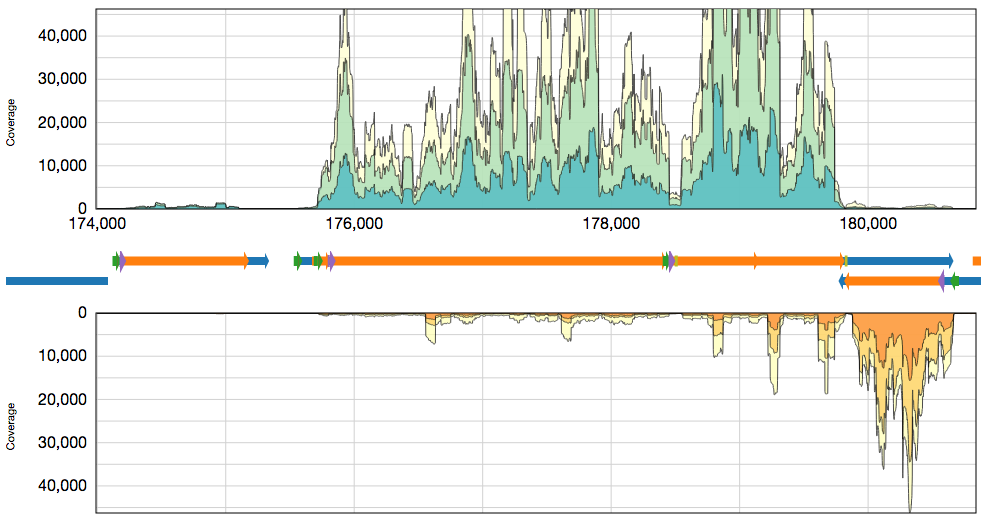
\includegraphics[width=\textwidth,height=2.5in]{images/Assembly/Sol/Sol-locus.png}
\subcaption{Sol locus}\label{fig:1a}}
% \label{fig:1}
\caption{Sol Locus: The Sol operon} This operon (\subref{fig:1a}) upper track) consists of OrfL, alcohol dehydrogenase (AdhE), and Co-A transferases A and B (ctfA,ctfB). SolR (far left) and acetoacetate decarboxylase (ADC; \subref{fig:1a} lower track, right) are also shown. Coverage for the Watson and Crick strands (top and bottom tracks) are visualized with an annotation track (center). Tracks show cumulative coverage for unstressed (yellow), butanol (light green/ light orange), and butyrate (green/orange) stressed samples over all time points. Transcripts (blue), ORFs (orange), RBSes (purple), inverted repeats (yellow), promoters (green), and TSSes (red) are represented as arrows and bars.
\end{figure}

The assembly suggests a distal transcription start site for the Sol operon at 175,564, agreeing with two previous studies of this region. Several increases in coverage are observed just after the proximal promoter as well. It is understood that the proximal promoter is the most active promoter motif for the Sol operon and this view is supported by our data. The assembly also shows a distinct transcription start site for SolR, in agreement with previous findings. The coverage data also agree with the single transcription start site for Adc, shown as a distinct increase in coverage. However, some remediation is required in the case of the Adc transcription start site and the 3' UTR of the Sol operon, which have been fused to residual signal from neighboring loci. This is the first example of misassembly, which I will address in the next section.
% Transcription start sites SOL Fig 2.
\begin{figure}
\small
{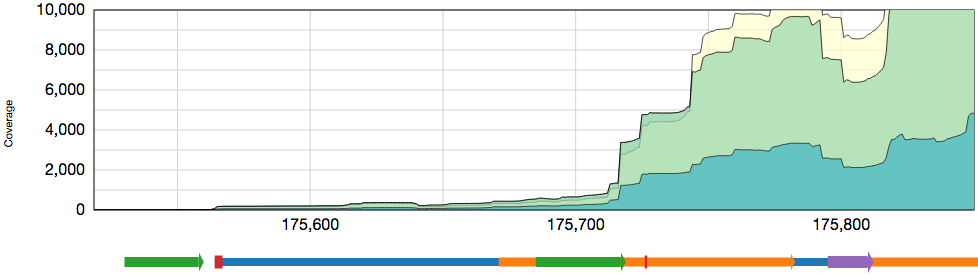
\includegraphics[width=\textwidth,height=1.5in]{images/Assembly/Sol/Sol-TSS.png}
\subcaption{Sol operon transcription initiation region. The distal (left) and proximal (right) transcription start sites (red) are shown for AdhE (far right, orange).}\label{fig:2a}}
{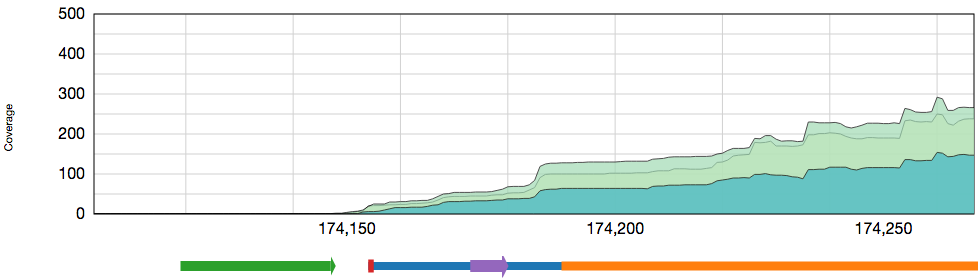
\includegraphics[width=\textwidth,height=1.5in]{images/Assembly/Sol/Sol-SolR-TSS.png}
\subcaption{SolR transcription initiation region}\label{fig:2b}}
{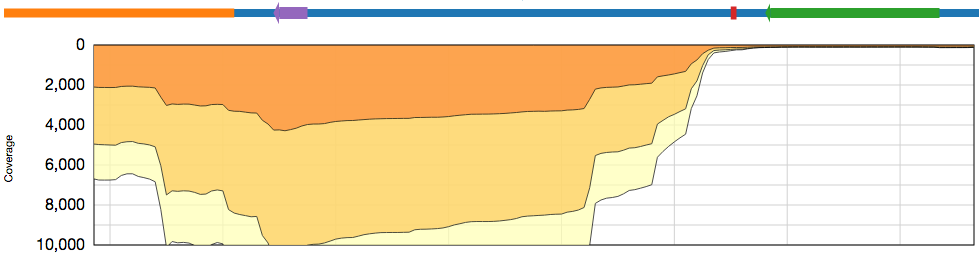
\includegraphics[width=\textwidth,height=1.5in]{images/Assembly/Sol/Sol-Adc-TSS.png}
\subcaption{Adc transcription initiation region on the Crick strand.}\label{fig:2c}}
%\label{fig:1.5}
\caption{Sol Locus Transcription Start Sites} \subref{fig:2a}) Sol operon (OrfL, center; AdhE right) transcription start sites. The coverage and assembly data have strong agreement with previously described proximal and distal promoters and transcription start sites. \subref{fig:2b}) The assembled transcription start site for SolR agrees with previous findings. \subref{fig:2c}) Transcription initiation region for Adc. While the coverage clearly shows the appropriate increase, the transcription start site has been fused to residual coverage upstream of the true TSS. 
\end{figure}
% Transcription stop sites      Fig 3.
\begin{figure}
{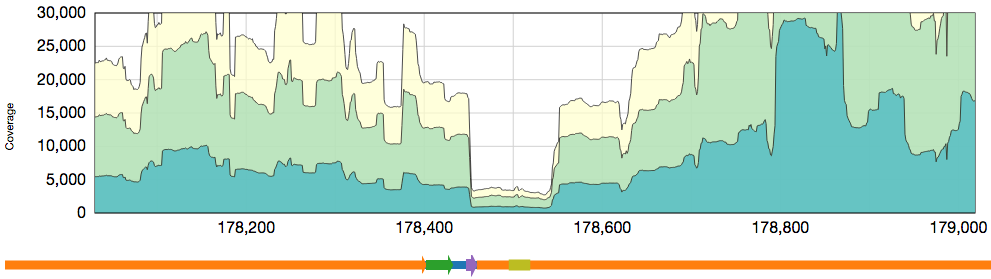
\includegraphics[width=\textwidth,height=1.5in]{images/Assembly/Sol/Sol-AdhE-terminator.png}
\subcaption{Putative AdhE (left) terminator, CtfA (right) promoter}\label{fig:3a}}
{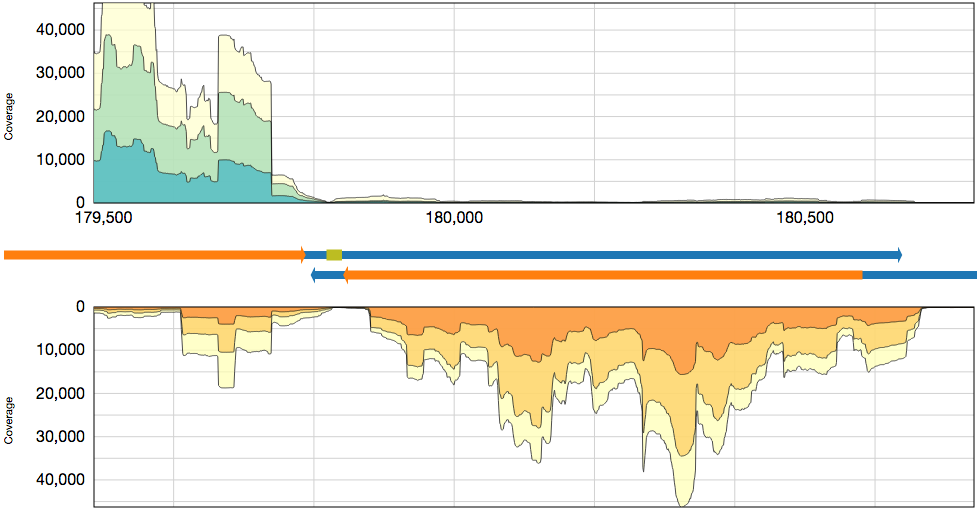
\includegraphics[width=\textwidth,height=2.5in]{images/Assembly/Sol/Sol-bifunctional-terminator}
\subcaption{Bifunctional Rho-independent terminator for Sol operon (upper track, left), Adc}\label{fig:3b}}
\caption{Sol Locus Transcription Stop Sites}
 \subref{fig:3a}) Low coverage in the Sol operon. A terminator may be partially responsible for a sustained low coverage level in the Sol operon. Additionally, a promoter motif was located upstream of the CtfA RBS and the pattern of expression is consistent with these observations. \subref{fig:3b}) A bifunctional terminator, likely responsible for transcriptional termination of both Adc and the Sol operon.
\end{figure}

The depth of coverage is also fairly consistent across these regions, except for a ~100bp region near the N-terminus of CtfA. This decrease in coverage can be explained by an inverted repeat present in this region, which could be difficult to sequence. The terminator sequence had a \(\Delta\)G of approximately -8kcal/mol, not as strong as the -12kcal/mol terminator at the end of the Sol operon. It is also interesting to note that a promoter motif TTCATA(13)TATAAT is also present in the region, upstream of the RBS. Primer extension studies for this operon frequently use probes from AdhE, at the exclusion of CtfA. Additionally, most Northern blot analyses of this region follow the work of Durre et al, where probes were only designed for AdhE. In one source (Fontaine, JBac 2002), a faint band is visible for a ~2.6kb RNA, which matches reasonably to the 2.7kb continuous sequence that we observe for AdhE in this example. Unfortunately, many other studies of this locus use AdhE probes exclusively and/or have sliced or semi-quantified their blots for publication, preventing further investigation of alternate bands. It is possible that 3 or more transcripts exist for this locus: the first being the whole operon, the second being AdhE on its own, and the third containing CtfA and CtfB.

In summary, this example demonstrates the accuracy of this technique in locations of the genome where residual signal is minimal or absent. Additionally, the need for additional annotation information such as promoters and terminators provides context for the coverage and assembly. Finally, the Sol operon demonstrates the need for semi-automated solutions to the issue of extended transcripts. In the case of Adc, the assembled transcription start site extends beyond the known start site, promoter, and coverage signals. We will see in future examples that coverage alone does not always identify the correct transcription start site and can be misleading in some cases. The next example involves another pair of solventogenic genes, the butanol dehydrogenases.



This Bdh region encodes two butanol dehydrogenase enzymes. These enzymes catalyze the final redox reaction between the fementation intermediate butyryl-CoA and NAD[P](H\textsuperscript{+}). Despite their name, these enzymes are capable of reducing both acetyl and butyryl groups but have widely different specificities for these substrates. I wanted to understand how this dataset is able to capture the transcription start sites for this location, which also has primer extension experiments that have determined that transcription start site for this region.

The BdhA and BdhB transcripts display a pattern of coverage consistent with previously published transcript sizes, start sites, promoters, and terminators. The assembly has captured the transcription start site of BdhA very well, but fails to capture the full length of the ORF and transcript, with respect to the hairpin annotation and coverage data. In contrast, the coverage of the BdhB gene captures the transcript boundaries very well, but the assembly has failed to produce its two boundaries exactly. In these two cases, determining the true boundaries of these transcripts benefits from promoter and terminator predictions, ORF annotation, and the coverage information for the transcript.

In this example, the BdhA and BdhB transcripts were very close to capturing the true boundaries of these genes. In the case of BdhA the TSS was precise, but the assembled transcript did not match the coverage pattern or the ORF and terminator annotations. This issue may be simpler to resolve computationally, compared with the issue of the two extended transcripts observed in the Sol locus and the extended 5' and 3' UTRs of the BdhB gene. Fortunately, the next example is another positive example, this time of a stress-response operon containing the heat-shock proteins GroES and GroEL.
%         BDH LOCUS          Fig 4.
\begin{figure}
\small
{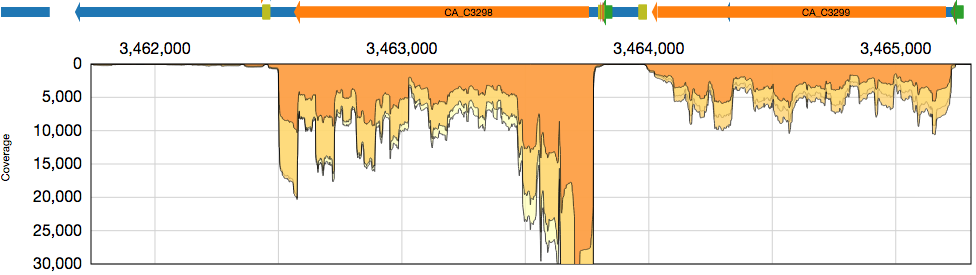
\includegraphics[width=\textwidth,height=1.5in]{images/Assembly/Bdh/Bdh-locus.png}
\subcaption{BdhB(left) and BdhA(right) on the negative strand. Features are colored as above.}\label{fig:4a}}
{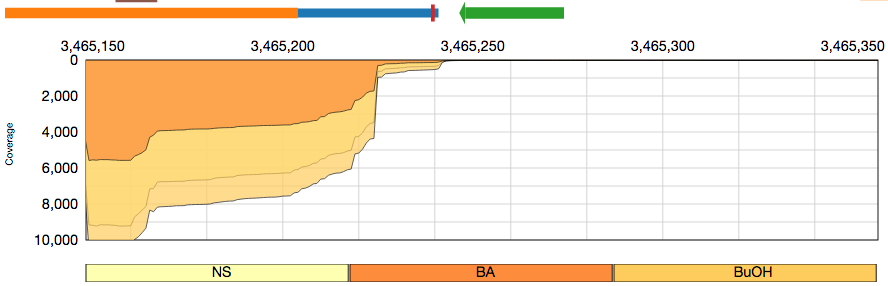
\includegraphics[width=\textwidth,height=1.5in]{images/Assembly/Bdh/BdhA-TSS.png}
\subcaption{BdhA Transcription Initiation Region}\label{fig:4b}}
{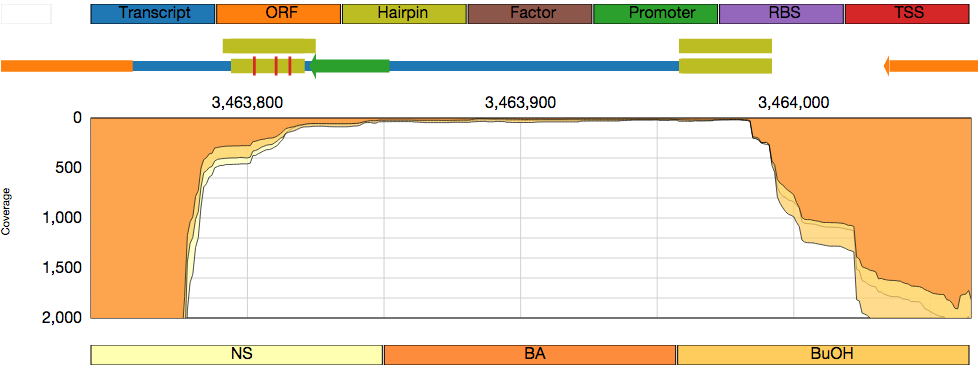
\includegraphics[width=\textwidth,height=1.5in]{images/Assembly/Bdh/BdhB-TSS.png}
\subcaption{BdhB Transcription Initiation Region}\label{fig:4c}}
\caption{Bdh Locus and Transcription Start Sites}
\subref{fig:4a}) Both genes in this locus produce distinguishable coverage patterns, and the coverage pattern and assembly agree to a good extent. It is worth noting the trailing 3' UTR after the BdhB ORF and hairpin. Additionally, the BdhA transcript (blue arrow, right) terminates before the end of the ORF and the hairpin. These two regions require minor corrections. \subref{fig:4b}) The BdhA transcript displays a sharp increase in coverage near the transcriptional start site. This data agrees to a good extent with primer extension studies for this gene. \subref{fig:4c}) The BdhB also contains a sharp increase in coverage near the published transcription start site. However, the assembled transcript extends to the nearby terminator. This region also requires minor correction.
\end{figure}

The GroES and GroEL proteins are heat-shock responsive chaperonins that are required for robust growth at all temperatures. The proteins are highly conserved across all species and are expressed in \textit{C. acetobutylicum} on a 2.15kb transcript, a length consistent with previous studies. These proteins are an integral part of the solvent stress response and the broader stress response systems of this and other bacterial species. A single strong terminator is present at the end of the transcript and a promoter motif upstream of the start site was found previously. The observed transcript coordinates are also consistent with previous studies. This example shows the coordinates of this operon reproduced faithfully. In the next example we will see the Spo0A locus, fused in a massive transcript with the surrounding signal. We will also see an interesting benefit of semi-automated curation.
\begin{figure}
\small
{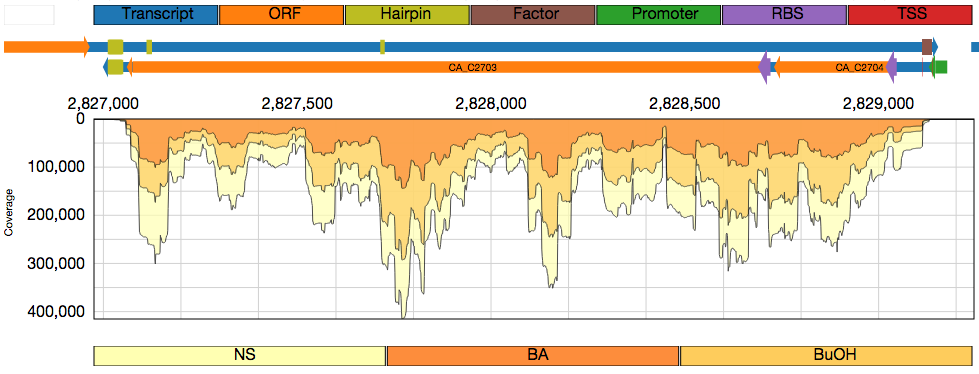
\includegraphics[width=\textwidth,height=1.5in]{images/Assembly/GroESL/GroESL-locus.png}
\subcaption{GroEL (left) and GroES (right) on the negative strand.}\label{fig:5a}}
{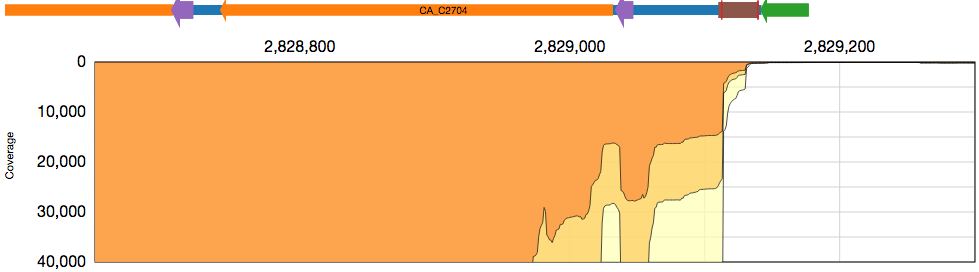
\includegraphics[width=\textwidth,height=1.5in]{images/Assembly/GroESL/GroESL-TSS.png}
\subcaption{GroES/EL operon transcription initiation region}\label{fig:5b}}
\caption{GroES/EL Locus and Transcription Initiation Region}
\subref{fig:5a}) GroES and GroEL form an operon that is responsive to heat-shock through a derepression mechanism.
\end{figure}

Spo0A is the master regulator of sporulation and stationary phase phenomena. This protein is thought to ultimately transduce growth-limiting and stressful signals into sporulation behavior in a number of anaerobic firmicutes. In previous studies, Spo0A was shown to be translated from a 0.9kb transcript in \textit{C. acetobutylicum}. Here we observe a slightly longer transcript of ~1.1kb according to the pattern of coverage. However, no Rho-independent terminators were found immediately downstream (\textless  200bp) of Spo0A, suggesting either a non-intrinsic termination mechanism or differing transcript sizes from those previously reported. Unfortunately, the boundaries represented by this coverage pattern were not detected due to the background signal in the area. Consequently, this region needs some remediation and is the first example of a completely fused transcript, not merely an extension.

In a nearby location, the genes CAC2073-2078 are found in a tight grouping near a large peak of expression. This peak correpsonds to an uncharacterized protein CAC2079 that is present in UniProt but absent from NCBI and KEGG databases. Its coverage appears to be largely above 20k per base, independent of the surrounding regions (although the transcript is indeed fused). Bioinformatic analysis suggests that it shares sequence similarity to proteins in the \textit{Clostridia}, \textit{Bacilli}, \textit{Baceteroidetes}, and \textit{Halobacteria}. While there was no common catalytic or active domain unifying this group of homologs, the region of homology tends to precede a transmembrane motif. Further analysis via PSI-blast result suggests sequence similarity to mATE (Multidrug And Toxic-compound Extrusion) efflux family proteins. mATE family proteins use electrochemical gradients to export antibiotics and other toxic compounds. The data suggest that the expression of this protein is important to \textit{C. acetobutylicum} and it will be interesting to examine the expression profile statistically. This instance demonstrates the synergy of older annotations with the newer coverage data and once again the need for semi-automated curation. Next we explore another stress-responsive region with a regulatory protein, the HrcA locus.

\begin{figure}
\small
{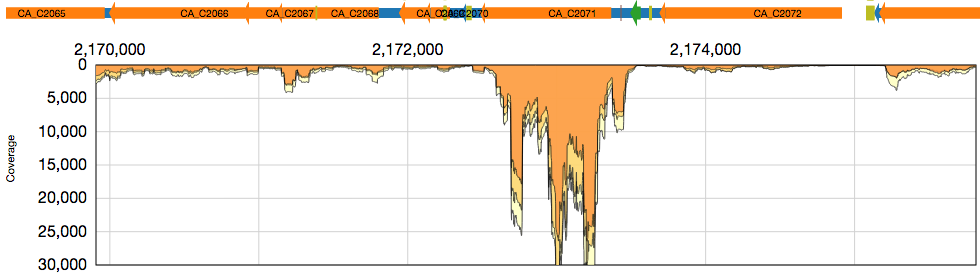
\includegraphics[width=\textwidth,height=1.5in]{images/Assembly/Spo0A/Spo0A-locus.png}
\subcaption{Spo0A transcript (center) fused to signal from neighboring regions}\label{fig:6a}}
{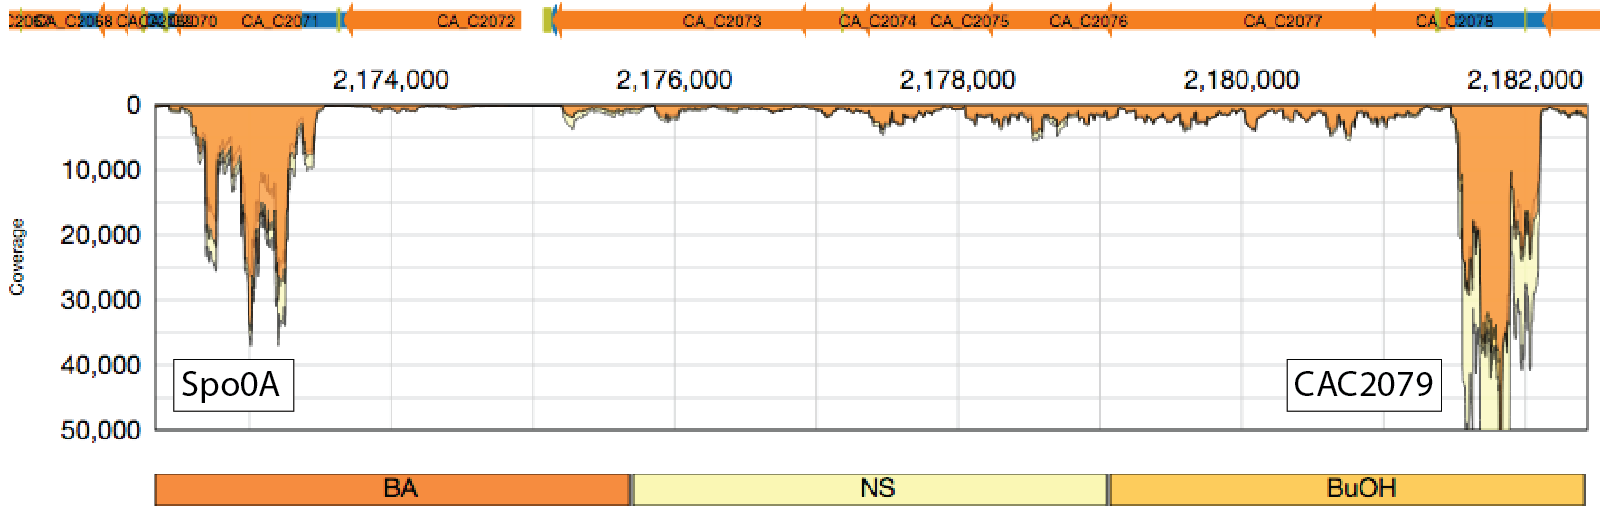
\includegraphics[width=\textwidth]{images/Assembly/Spo0A/CAC2079.png}
\subcaption{Upstream region of Spo0A, including CAC2079, a putative protein missing from many databases.}\label{fig:6b}}

\caption{Spo0A locus}
\subref{fig:6a}) The Spo0A transcript is found in a region of sufficient k-mer complexity and background coverage for the assembled transcript to be fused to signal from neighboring operons. This region clearly requires attention from curation strategies. \subref{fig:6b}) The region upstream of Spo0A consists of a late stage sporulation protein and a group of proteins in tight formation. Interestingly, there is a missing annotation in NCBI and KEGG for protein CAC2079 near a large peak of expression, in between the annotated proteins CAC2078 CAC2080.
\end{figure}

The HrcA locus consists of a polycistronic operon with multiple transcription start sites. The operon consists of the heat-shock program regulator HrcA, the nucleotide exchange factor GrpE, and the molecular chaperones DnaK and DnaJ. In an early study of this region, 4 transcripts were identified for this operon. The first was a 5kb transcript containing all 4 proteins. The second a 3.8kb transcript contains HrcA, GrpE, and DnaK while the third (2.6kb) contains only GrpE and DnaK. The final transcript contains DnaJ and is 1.4kb. One previously documented Rho-independent terminator has been described downstream of DnaK in \textit{C. acetobutylicum}.

In this dataset, the coverage pattern matches very well with the previously published transcript size of 5kb. Interestingly, the HrcA transcription start site determined by the uncurated assembly is comparable to previous studies. Moreover, the assembly predicts a transcription start site with reasonable accuracy, considering the level of residual signal from the upstream gene. The data could certainly reflect the transcriptional terminator downstream of DnaK, but no Rho-independent terminator was found downstream of DnaJ using three different algorithms. The termination of this transcript may be due to a non-intrinsic termination mechanism. This region has also been fused to signal from the downstream gene.

\begin{figure}
\small
{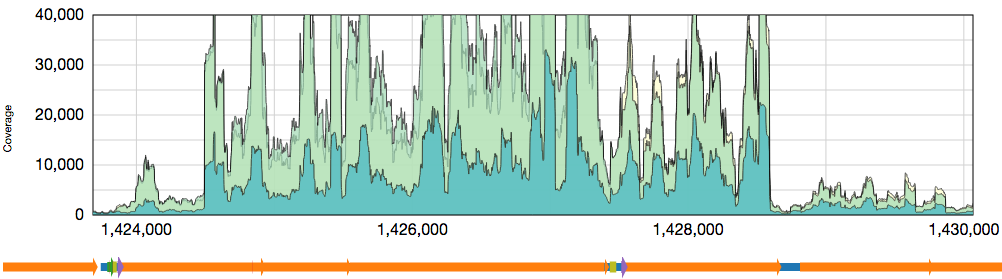
\includegraphics[width=\textwidth,height=1.5in]{images/Assembly/HrcA/HrcA-locus.png}
\subcaption{Operon consisting of HrcA, GrpE, DnaK, and DnaJ}\label{fig:7a}}
{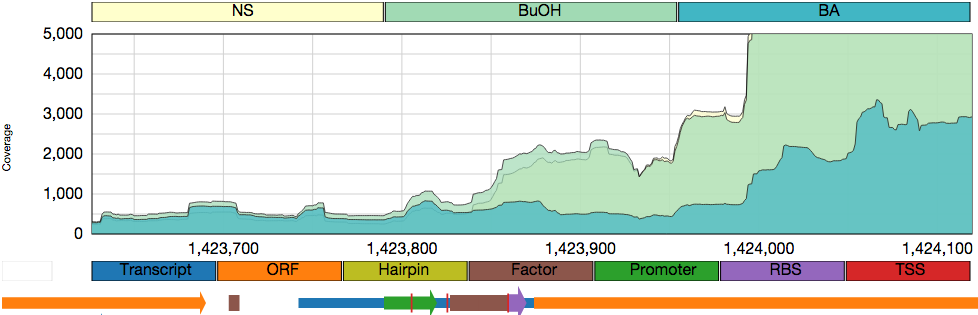
\includegraphics[width=\textwidth,height=1.5in]{images/Assembly/HrcA/HrcA-TSS.png}
\subcaption{HrcA transcription initiation region.}\label{fig:7b}}
{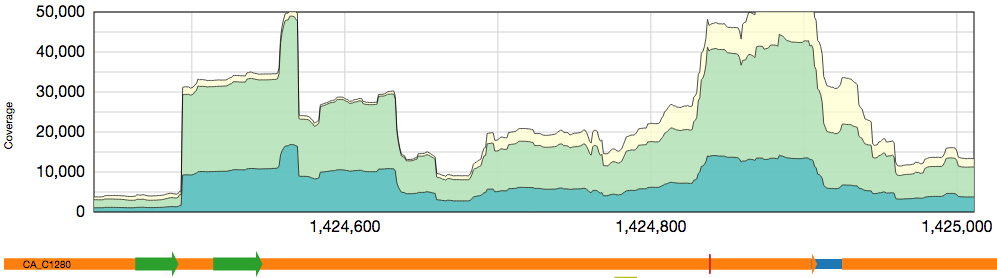
\includegraphics[width=\textwidth,height=1.5in]{images/Assembly/HrcA/GrpE-TSS.png}
\subcaption{GrpE transcription initiation region.}\label{fig:7c}}
{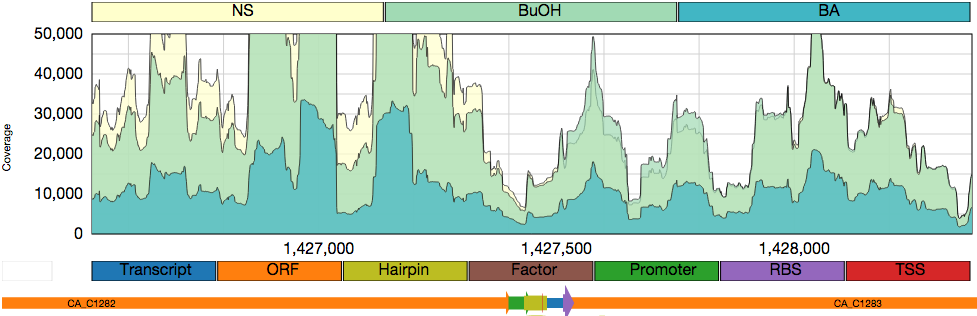
\includegraphics[width=\textwidth,height=1.5in]{images/Assembly/HrcA/DnaKJ-IGR.png}
\subcaption{DnaK-DnaJ IGR and DnaJ transcription initiation region}\label{fig:7d}}
\caption{HrcA locus}
\subref{fig:7a}) The highly expressed HrcA locus encodes several transcripts of different size. \subref{fig:7b}) The assembled transcription start site for the HrcA gene provides a reasonable estimate, considering the level of background signal for this region. \subref{fig:7c}) The transcription start site is not distinguishable in the coverage data. \subref{fig:7d}) The intergenic region between DnaK and DnaJ contains the only hairpin for this operon, which matches a decrease in coverage. The reported transcription start site is not identifiable from the coverage in this region.
\end{figure}

\subsection{Identify and Attempt to Resolve Remaining Issues}
There are two principal challenges relating to this uncurated transcriptome assembly. The first relates to the qualification of novel transcripts which I will defer to a later time. The second involves the curation of the 1057 transcripts which encode reference CDSes. After considering the examples above, we are left with a few types of misassembly to address.
\begin{enumerate}
\item Partial transcripts which overlap reference ORFs, but do not completely contain them. (e.g. BdhA)
\item Extended transcripts that possess larger UTRs than would be expected with respect to promoter and terminator motifs and coverage patterns. (e.g. Adc, CtfA/B)
\item Fused transcripts where the transcript from one gene is completely fused with signal from neighboring loci, with respect to prior knowledge, promoter, and terminator motifs (e.g. Spo0A).
\end{enumerate}

The first issue requires the simple solution of adjusting the transcript boundaries to include reference ORFs where there is not complete inclusion. Practically this requires only some minimal scripting and the use of '\href{http://bedtools.readthedocs.org/en/latest/content/tools/merge.html}{merge}' from bedtools, a toolkit for genomic set operations. The second issue requires a slightly more complicated solution of integrating information of regulatory motifs, terminators, and coverage information to find the solution that produces the most agreement between these various sources. In practice, I will integrate the various sources in the genome browser for context with the coverage information from this experiment. No completely automated tools exist to accomplish this. However, on average each transcript requires only a minimal amount of decision and should in principle be easy to curate. The third type of gene is completely fused to signal from other genes or noise. In the case of Spo0A, the true signal was simple to distinguish from noise, even in the absence of a Rho-independent terminator. In other cases the solution may not be so simple but contextual information about ontology combined with the various signals of coverage and stress response, promoters, and terminators make the problem more tractable. 

In principle, each of the pieces of information that I will integrate will not reproduce the transcript boundary on its own. In the examples above there are instances where the coverage alone fails to describe the transcript boundary, while the linguistic complexity of the dataset, used by the assembly algorithm, reproduces the boundary to a good extent. In other instances the opposite is true: a dramatic change in coverage near terminators or other signals is not recognized by the assembly alone. For that matter, there appear to be instances of non-intrinsic termination to complicate matters further. Therefore, these information are synergistic with respect to defining transcript boundaries and the absence of one signal may be made up for by the presence of another.

\subsection{Novel Transcripts}

\subsection{Exploratory Tools}


